Полигон - квадратное поле $3200\times3200$ мм., разделенное на квадратные сектора $400 \times 400$ мм.
Некоторые сектора отделены друг от друга перегородкой высотой $100$ мм.
Некоторые сектора недоступны для посещения робототехническим устройством и представляют из себя 
модель стеллажа высотой $210$ мм.
На каждой полке стеллажа располагается черный контейнер с грузом ~(рис.~\ref{fig:container}) размером
$200 \times 300 \times 100$ мм (груз - 2-3 коробки~(рис.~\ref{fig:box}) размером $180 \times 80 \times 85$ мм).


\begin{figure}[h]
\begin{center}
\begin{minipage}[h]{0.5\linewidth}
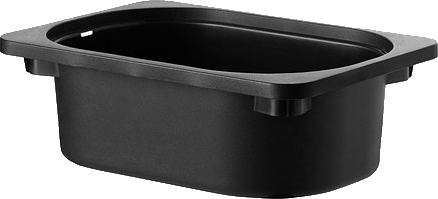
\includegraphics[width=1\linewidth]{sources/container}
\caption{Внешний вид контейнера}
\label{fig:container} 
\end{minipage}
\hfill 
\begin{minipage}[h]{0.4\linewidth}
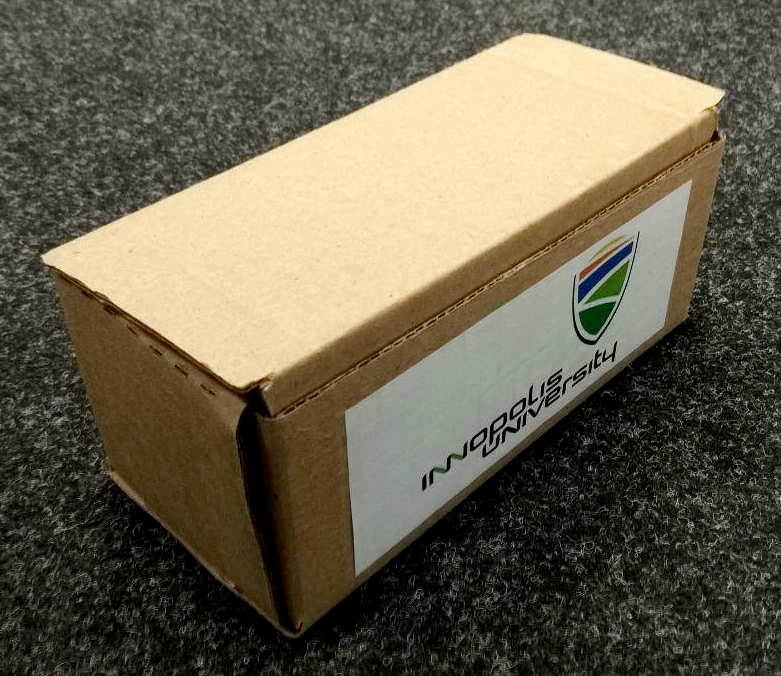
\includegraphics[width=1\linewidth]{sources/box}
\caption{Внешний вид коробки}
\label{fig:box}
\end{minipage}
\end{center}
\end{figure}

Полигон окружен бортом высотой $100$ мм.
Конфигурация полигона определяется в первый день финального этапа и объявляется участникам.
Данная конфигурация будет использоваться во все дни финального этапа.

На нижней полке стеллажа, прилегающего одной из четырех сторон к сектору сервисного обслуживания,
на высоте от 100-150 мм от уровня поверхности поля закреплен ARTag маркер (\url{https://goo.gl/WaTFMB}),
определяющий номер робота и координаты сектора приписки (сектор финиша для конкретного робота).
Размер маркера - $30\times30$ мм.
Маркер обращен лицевой стороной внутрь сектора сервисного обслуживания, координаты которого известны заранее.
Конкретная высота расположения маркеров определяется в первый день финала и остается
постоянной во все дни финального этапа. При этом допустимая погрешность установки
маркеров $\pm 5$ мм. Пример расположения маркера на стелаже представлен на рисунке \ref{fig:cellInARTag}

\putImgForRef{8cm}{sources/cell-with-ARTag.jpg}
{Стеллаж с установленным ARTag маркером}{fig:cellInARTag}

Маркер состоит из $6\times6$ элементов одинакового размера.
Элементы маркера, расположенные по его границе --- всегда черные. Четыре элемента,
находящиеся в углах внутреннего $4\times 4$ квадрата определяют ориентацию маркера таким
образом, что только один из них --- белый.
Оставшиеся $12$ элементов маркера кодируют число по следующему правилу: если элемент черный, то в он обозначает $1$, если белый,
то $0$ при этом самый первый элемент --- старший бит закодированного числа.
Нумерация элементов относительно ориентационных элементов обозначена на рисунке \ref{fig:marker-bits}.

\putImgForRef{5cm}{sources/artag-about}
{Нумерация элементов маркера относительно ориентационных элементов}{fig:marker-bits}


\putImgForRef{5cm}{sources/artag-ex1}
{Маркер с закодированным значением - $010011100101_2$}{fig:marker-ex1}


Закодированное на маркере двоичное двенадцатибитное число закодировано с использованием кода Хэмминга (https://habr.com/ru/post/140611/), в котором 8 информационных битов
и 4 контрольных бита:
\begin{enumerate}
    \item[1] Первый контрольный бит;
    \item[2] Второй контрольный бит;
    \item[3] Старший бит номера робота $N$($1 \leq N \leq 3$);
    \item[4] Третий контрольный бит;
    \item[5] Младший бит номера робота $N$($1 \leq N \leq 3$);
    \item[6] Первый (старший) бит координаты $X$ робота $N$ ($0 \leq X_N \leq 7$);
    \item[7] Второй бит координаты $X$ робота $N$ ($0 \leq X_N \leq 7$);
    \item[8] Четвёртый (последний) контрольный бит;
    \item[9] Третий (младший) бит координаты $X$ робота $N$ ($0 \leq X_N \leq 7$);
    \item[10] Первый (старший) бит координаты $Y$ робота $N$ ($0 \leq Y_N \leq 7$);
    \item[11] Второй бит координаты $Y$ робота $N$ ($0 \leq Y_N \leq 7$);
    \item[12] Третий (младший) бит координаты $Y$ робота $N$ ($0 \leq Y_N \leq 7$);
\end{enumerate}


Маркер на рисунке \ref{fig:marker-ex1} кодирует число $010011100101_2$ --- $N = 1$, $X = 6$, $Y = 5$.
Таким образом, сектор приписки для робота $1$ находится в позиции с координатами $(6, 5)$ --- см. рисунок \ref{fig:sector-example}.


\putImgForRef{9cm}{sources/sector-example}
{Расположение сектора финиша для маркера из рисунка \ref{fig:marker-ex1}}{fig:sector-example}

Гарантируется, что сектора сервисного обслуживания будут располагаться в таких
местах полигона, где к сторонам сектора прилегает как минимум один стеллаж.

Сектора активаций роботов (стартов), сектора сервисного обслуживания и сектора приписки никак
не обозначаются на поле и определяются непосредственно перед каждым заездом робота.

